\section{Avaliação com protótipo real no PlanetLab}
\label{sec:deploy}

Nesta seção avaliamos um protótipo do \rmprt{} no PlanetLab.
Implantamos o Paris traceroute e o \rmprt{} em 140 nós PlanetLab e
coletamos medições por 18 horas de 30 de Novembro de 2012.  Cada nó
executa o Paris traceroute para medir caminhos periodicamente.  Como no
conjunto de dados utilizado nas seções anteriores, cada nó monitora
caminhos para 1.000 destinos escolhidos aleatoriamente de uma lista com
34.820 destinos alcançáveis na Internet.  Quando duas medições
consecutivas com Paris traceroute detectam uma mudança, executamos o
\rmprt{} para remapeá-la.  Cada nó leva em média 7~horas e 42~minutos
para medir os 1.000 caminhos.  Devido à baixa frequência de sondagem,
este conjunto de dados contém apenas 87.848 mudanças.  Os caminhos
medidos atravessam 7.143 sistemas autônomos e 95\% dos sistemas
autônomos de grande porte na Internet~\cite{oliveira08as2tier}.

A \figstr~\ref{fig:deploy.savings} mostra a redução do custo de
remapeamento quando usamos o \rmprt{} em vez do Paris traceroute.
Comparando com a \figstr~\ref{fig:sim.savings.cmp}, a redução média do
custo de remapeamento no cenário real é quantitativamente similar aos
resultados obtidos via simulação (linha sólida).  Por exemplo, reduzimos
pra menos da metade o custo de remapeamento de 90\% das mudanças de
caminho no cenário real.

A redução de custo para rotas curtas e longas é mais similar à redução
de custo geral no cenário real que nas simulações.  Em outras palavras,
as linhas tracejadas na \figstr~\ref{fig:deploy.savings} estão mais
próximas da linha sólida que na \figstr~\ref{fig:sim.savings.cmp}.
Atribuímos essa mudança a três fatores: (i) o menor número de mudanças
observadas no cenário real pode limitar a variedade de mudanças
observadas; (ii) diferenças no conjunto de caminhos monitorados; e (iii)
a diferente forma de detecção de mudanças (os dados utilizados nas
simulações foram coletados com o \dtrack{}).

A \figstr~\ref{fig:deploy.latency} mostra os $25^o$, $50^o$ e o $75^o$
percentis da latência de remapeamento em função do número de saltos
sondados durante o processo de remapeamento.  Avaliamos a latência de
remapeamento por que o \rmprt{} sonda saltos sequencialmente: a decisão
do próximo salto a sondar depende do resultado do último salto sondado.
O Paris traceroute, em contrapartida, poderia paralelizar a sondagem de
saltos (apesar da implementação padrão não fazê-lo).  Como a maior parte
dos remapeamentos com \rmprt{} requer sondagem de poucos saltos
(\figstr~\ref{fig:sim.abs.cmp}), a latência de remapeamento geralmente é
menor que 5 segundos.  A \figstr~\ref{fig:deploy.latency.ptr} mostra os
$25^o$, $50^o$ e $75^o$ percentis da latência de remapeamento com Paris
traceroute no cenário real.  Nosso objetivo não é comparar a latência de
remapeamento do \rmprt{} com Paris traceroute, pois a latência é
diretamente afetada por decisões de implementação da ferramenta.  Nosso
objetivo é mostrar que a latência de remapeamento com \rmprt{} é
aceitável para uso em sistemas reais.  Notamos ainda que um sistema de
mapeamento topológico como o \dtrack{} pode executar o \rmprt{}
simultaneamente em caminhos diferentes caso mais de uma mudança seja
detectada num curto intervalo de tempo.

\begin{figure}
\begin{center}
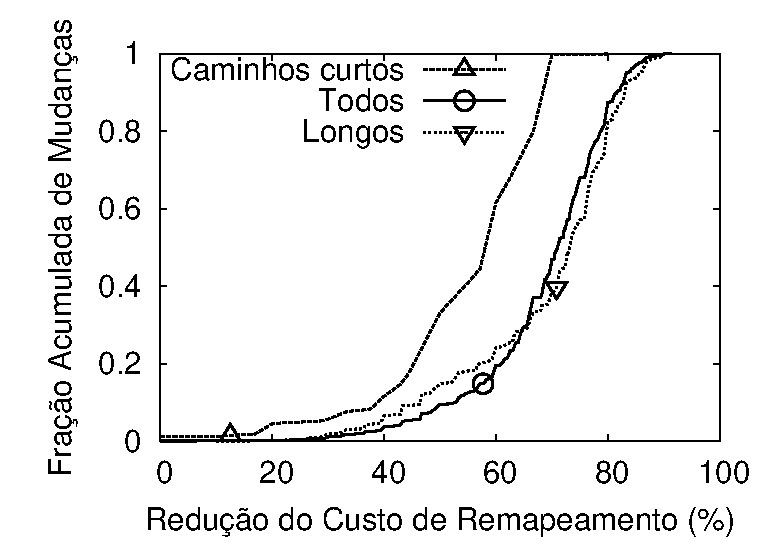
\includegraphics[width=0.47\textwidth]{figs/deploysavings.eps}
\caption{Redução do custo de remapeamento com \rmprt{} em cenários
reais.}
\label{fig:deploy.savings}
\end{center}
\end{figure}

\begin{figure}
\begin{center}
\subfigure[\rmprt{}]{
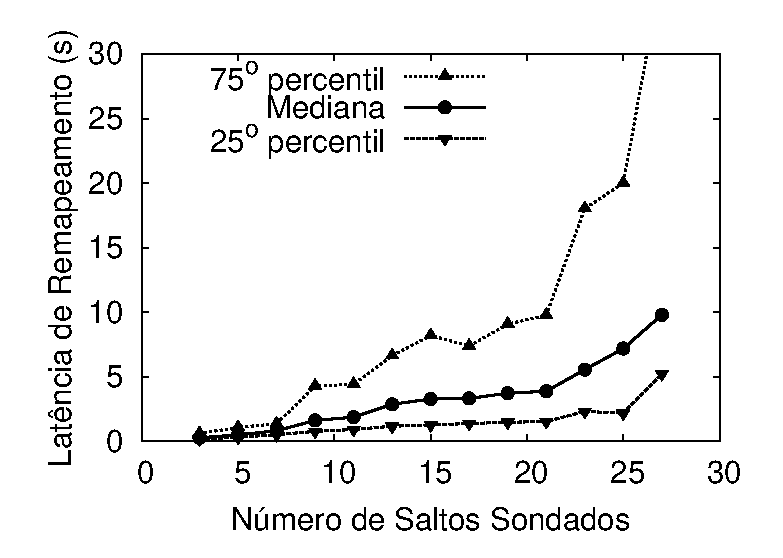
\includegraphics[width=0.47\textwidth]{figs/latency.eps}
\label{fig:deploy.latency}}
\hspace{2mm}
\subfigure[Paris traceroute]{
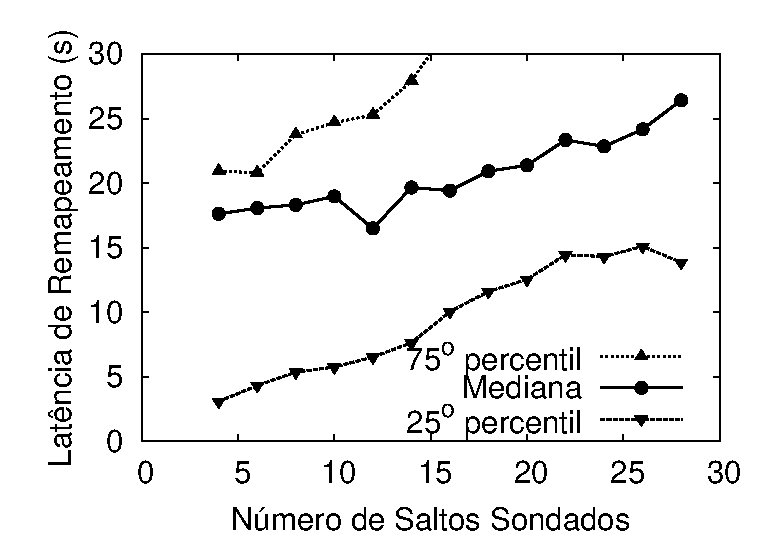
\includegraphics[width=0.47\textwidth]{figs/ptrlatency.eps}
\label{fig:deploy.latency.ptr}}
\caption{Latência de remapeamento em cenários reais.}
\end{center}
\end{figure}

Por último, avaliamos se o remapeamento com o \rmprt{} é equivalente a
utilizar o Paris traceroute para medir o novo caminho por inteiro.  Para
cada mudança observada no cenário real, comparamos os saltos remapeados
pelo \rmprt{} com a rota medida pelo Paris traceroute.  Apenas 0,6\% das
medições com \rmprt{} são diferentes das medições com Paris traceroute.
A identificação de roteadores que fazem balanceamento de carga usando
Paris traceroute ou \rmprt{} é probabilística~\cite{veitch09balancer}.
Por exemplo, a configuração padrão do Paris traceroute e do \rmprt{}
identifica todos os roteadores que fazem balanceamento de carga numa
rota com 95\% de confiabilidade.  Erros de medição são inevitáveis e
causam diferenças entre remapeamentos independente da ferramenta
utilizada.  Outra causa para diferença nos remapeamentos são mudanças de
roteamento que acontecem no intervalo entre a medição com Paris
traceroute e a medição com \rmprt{}.

Sumarizando, o remapeamento de mudanças de caminho na Internet com
\rmprt{} é tão preciso quanto remapeamento com Paris traceroute, reduz
significativamente o número de sondas enviadas e tem pouco impacto na
latência de remapeamento.

